\section {EPICS Archiver Appliance}
\label{sec:archiver}
\subsection {Introdução}

O EPICS \textit{Archiver Appliance}, desenvolvido pelo instituto americano
\textit{National Accelerator Laboratory (SLAC)}, é capaz de monitorar e arquivar
um grande número de váriaveis, geradas por servidores
EPICS presentes na rede. O sistema fornece também opções de configuração de um
largo conjunto de parâmetros referentes ao armazenamento e monitoramento. Uma
\textit{appliance} é composta basicamente por quatro módulos distintos, sendo eles:

\begin{itemize}
  \renewcommand\labelitemi{--}
  \item \textit{Management}: provê as ferramentas necessárias para a gerência
  da \textit{appliance}. Permite, por exemplo, adicionar ou remover \textit{PVs}
  à lista de variáveis a serem arquivadas;
  \item \textit{Engine}: realiza a integração entre os módulos;
  \item \textit{Data Retrieval}: módulo responsável por recuperar os dados das
  \textit{PVs} arquivadas;
  \item \textit{ETL}: responsável por extrair os dados e tranformá-los a fim de
  que as aplicações possam processá-los posteriormente;
\end{itemize}

% A figura \ref{fig:epics_archiver} esquematiza o modo de funcionamento do
% \textit{EPICS Archiver Appliance}.
% 
% \begin{figure}[h]
%     
%     \centering
%     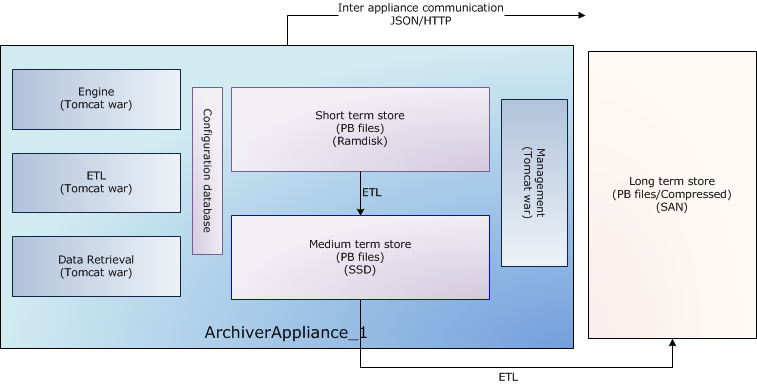
\includegraphics[scale=0.6]{image/applarch}
%     \caption {Modo de funcionamento de uma \textit{appliance}. Extraída de
%     \cite{archiver}.}
%     \label{fig:epics_archiver} 
% \end{figure} 

O instituto desenvolvedor da aplicação sugere que cada módulo seja lançado em
sua própria instância \textit{Tomcat}. Em adição, ele propõe a divisão da
unidade de armazenamento em 3 outras unidades, de acordo com a frequência em que
os dados são salvos. Essas unidades são divididas em \textit{short-term},
\textit{medium-term} e \textit{long-term storage}, cujas frequências de
armazenamento são, respectivamente, a cada hora, diária e anual. Essas
configurações podem ser modificadas através de arquivos
específicos, explicados nas próximas subseções.

\vspace{12pt}


Em um ambiente composto por diversos servidores EPICS e milhares de variáveis a
serem monitoradas, tal como o sistema de controle do \textit{Sirius}, um sistema
capaz de automatizar e agilizar o armazenamento e recuperação de dados se torna
fundamental para o monitoramento de eventuais problemas. Sendo assim, as próximas seções são
dedicadas à instalação e exploração dos recursos disponíveis nesta aplicação.

\subsection {Instalação}

A versão de Junho de 2016 do \textit{archiver} foi instalada no \textit{OPR23},
que se encontra na sala de controle, e pode ser acessada digitando-se o endereço
\texttt{10.0.4.69} em qualquer \textit{browser}. Atualmente, o arquivador possui
36 \textit{PVs} conectadas, contendo, inclusive, algumas das variáveis geradas
pelos receptores GPS, descritos na seção \ref{sec:pvsgps}. As próximas
subseções descrevem algumas das modificações realizadas no \textit{archiver}.

\subsubsection{\textit{Login} necessário}

Um dos principais problemas do arquivador é que qualquer pessoa logada
pode inserir ou remover variáveis do sistema. A fim de impedir que usuários não
autorizados realizem tais ações, modificou-se o código das
\textit{appliances} para verificar se o usuário foi autenticado com sucesso.
Para tal, instalamos um servidor LDAP no OPR23 e criamos uma página
de \textit{login}, acessada a partir de \url{http://10.0.4.69/login.html}. Quando o
usuário aperta o botão \textit{Ok}, uma requisição do tipo \textit{POST} é
enviada ao módulo \textit{PHP} que roda no servidor. Esse módulo consulta o LDAP
e retorna se o usuário foi autenticado ou não. Em caso de sucesso, uma nova
requisição do tipo \textit{POST} é enviada e capturada pelo módulo
\textit{management}, que, em seguida, inicia uma nova sessão para o usuário.
Enfim, antes de qualquer operação de inserção ou remoção de variáveis, o
módulo verifica se a sessão está definida e, caso esteja, autoriza a respectiva
operação. A intenção é integrar este sistema de \textit{login} ao servidor
LDAP do CNPEM no futuro.

\vspace{12pt}

Um usuário, denominado de \textit{Anônimo}, com permissões básicas de leitura é
disponibilizado por padrão e permite que qualquer pessoa consulte o
\textit{archiver} mesmo não estando autenticada.

\subsubsection{Mudanças no estilo}

Alguns arquivos \textit{css} (\textit{Cascading Style Sheet}) foram modificados
para refletir melhor o esquema de cores do laboratório. As imagens do
\textit{logo} também foram modificadas.

\subsection{Uso do CS-Studio no monitoramento} \label{appliance-csstudio}

O \textit{CS-Studio} \cite{css} pode ser usado para monitorar a
\textit{appliance}. Para isso, entre em \texttt{Edit \(>\) Preferences} e acesse
o item \texttt{CSS Applications \(>\) Trends \(>\) Data Browser}. No campo
\textit{Archive Data Server URLs}, adicione o endereço
\url{pbraw://10.0.4.69/lnls-control-archiver}.
Escreva qualquer \textit{Server alias}. Na tabela \textit{Default Archive Data
Sources}, adicione o mesmo endereço e aperte \textit{Ok} para salvar as
alterações.

\vspace{12pt}

É necessário alterar a perspectiva do \textit{CS Studio}. Acesse
\texttt{Windows \(>\) Open Perspective} e escolha \textbf{Data Browser}. Na aba
\textit{Archive Search}, escreva a \textit{URL} configurada anteriormente e no
campo \textit{Pattern}, escreva o nome das variáveis arquivadas que deseja
monitorar. Por exemplo, se escrevermos \texttt{Cnt:MikroE:*}, todas as variáveis
arquivadas para o receptor GPS da seção \ref{sec:pvsgps} poderão ser acessadas.
Clique com o botão direito na variável desejada e acesse \texttt{Process Variable \(>\) Data Browser}.

\subsection{Acessando a \textit{appliance} com \textit{Python}}

A \textit{appliance} pode ser acessada através de requisições \textit{JSON}
realizadas por um módulo escrito em \textit{Python}, por exemplo. Uma interface
gráfica foi implementada, usando os módulos \textit{Qt}, a fim de testarmos a
comunicação. Ela possui um gráfico, onde serão mostrados os dados recuperados,
uma caixa de opções, que possui todas as variáveis arquivadas na
\textit{appliance}, e componentes para seleção das datas de início e fim do
intervalo desejado. A figura \ref{fig:interface} representa o resultado da
implementação.

\vspace{12pt}

% \begin{lstlisting}[language=Python]
% import time
% import urllib2
% import json
% 
% class JsonRequester ():
%     
%     def __init__(self, data_retrieval_url, mgmt_url):
%         self.data_retrieval_url = data_retrieval_url
%         self.mgmt_url = mgmt_url
%     
%     def json_request_variables(self, variables_prefix):
%         
%         url_json = self.mgmt_url + 'bpl/getPVStatus?pv=' + variables_prefix
%         req = urllib2.urlopen(url_json)
%         data = json.load(req)
%         return data
%     
%     def json_request_data(self, variable, from_date, to_date):    
%         
%         retrieval_url = self.data_retrieval_url + "/data/getData.json?"
%         pv_name = ("pv=" + variable).replace(':', '%3A')
%         to_date =   ("&to=" + time.strftime("%Y-%m-%dT%H:%M:%S",to_date) + 
%         				".000Z").replace(':', '%3A')
%         from_date = ("&from=" + time.strftime("%Y-%m-%dT%H:%M:%S",from_date) + 
%         				".000Z").replace(':', '%3A')    
%         url_json = retrieval_url + pv_name + from_date + to_date
%         req = urllib2.urlopen(url_json)
%         data = json.load(req)
%         secs = [x['secs'] for x in data[0]['data']]
%         vals = [x['val'] for x in data[0]['data']]
%         return secs, vals
% \end{lstlisting}
% 
% O método construtor recebe 2 \textit{strings} como parâmetros.
% \textit{data\_retrieval\_url} e \textit{mgmt\_url} estão contidos no arquivo
% \textit{lnls\_appliances.xml} e representam, respectivamente, os endereços dos
% \textit{servlets} de obtenção de dados e gerenciamento da \textit{appliance}. A
% primeira \textit{url} será usada para recuperar os dados e a segunda, para obter
% as informações relativas às variáveis arquivadas.
% 
% \vspace{12pt}
% 
% O método \textit{json\_request\_variables} é responsável por retornar
% informações de uma ou várias variáveis, cujo nome (no caso de uma pesquisa de
% uma única variável) ou prefixo (parte comum ao nome de diversas variáveis) é
% passado como parâmetro. Para tal, utiliza o método \texttt{getPVStatus}, que é
% disponível no \textit{servlet} de gerenciamento e acessível via a \textit{url}
% \texttt{mgmt\_url}. Esse método também recebe como parâmetro nomes ou prefixos
% de variáveis, especificados após o trecho \texttt{pv=} na requisição
% \textit{json}. Para recuperar todas as variáveis arquivadas por uma
% \textit{appliance} que comecem com o prefixo \texttt{MBTemp}, por exemplo,
% bastar utilizarmos \texttt{pv=MBTemp*} na requisição. Uma vez construída a
% \textit{url}, é necessário utilizar as bibliotecas \textit{python}
% \texttt{urllib2} e \texttt{json}, que realizam a comunicação com os
% \textit{servlets}. 
% 
% \vspace{12pt}
% 
% O método \textit{json\_request\_data} retorna os dados arquivados para uma
% determinada variável, passada como parâmetro. Além dela, essa função recebe dois
% outros valores, sendo eles objetos do tipo \textit{time}, cuja implementação
% reside no módulo \texttt{time}. Esses parâmetros representam, por sua vez, as
% fronteiras do intervalo de tempo para o qual se deseja recuperar os dados, sendo
% que \texttt{from\_date} é a data mais antiga e \texttt{to\_date}, a mais
% recente. Se \texttt{to\_date} vale \texttt{None}, então o sistema o interpreta
% como o tempo no qual a chamada da função foi feita. Os dados são recuperados
% através do método \texttt{getData}, disponível no \textit{servlet}
% \texttt{retrieval} da \textit{appliance}. Antes de realizarmos a requisição, é
% necessário traduzir os objetos \textit{time} para o formato aceito pela
% servidor. Sendo assim, utiliza-se o método \texttt{strftime} do módulo
% \texttt{time} que retorna a representação \textit{string}, segundo a máscara
% especificada (no nosso caso, \texttt{\%Y-\%m-\%dT\%H:\%M:\%S}), do objeto
% passado como parâmetro. A requisição é, enfim, realizada através dos mesmos
% métodos que foram usados na função anterior.
% 
% \vspace{12pt}
% 
% O servidor envia todos os dados, isto é, valores e datas do respectivo evento,
% em único vetor de dicionários. Por este motivo, é necessário processarmos essa
% estrutura antes de retorná-la ao programa que chamou o método. Os valores são
% acessíveis pelo índice \texttt{val} e seu tipo depende da aplicação. A data dos
% eventos relativos aos valores são recuperados pelo índice \texttt{secs} e são
% números inteiros que contém o número de segundos desde uma data de referência
% (1 de Janeiro de 1970) usada no \textit{servlet}. É necessário notar que as
% datas retornadas estão em \textit{UTC}, portanto é exigido que tais
% valores sejam convertidos para a o fuso local.
% 
% \vspace{12pt}


\begin{figure}[h]
    
    \centering
    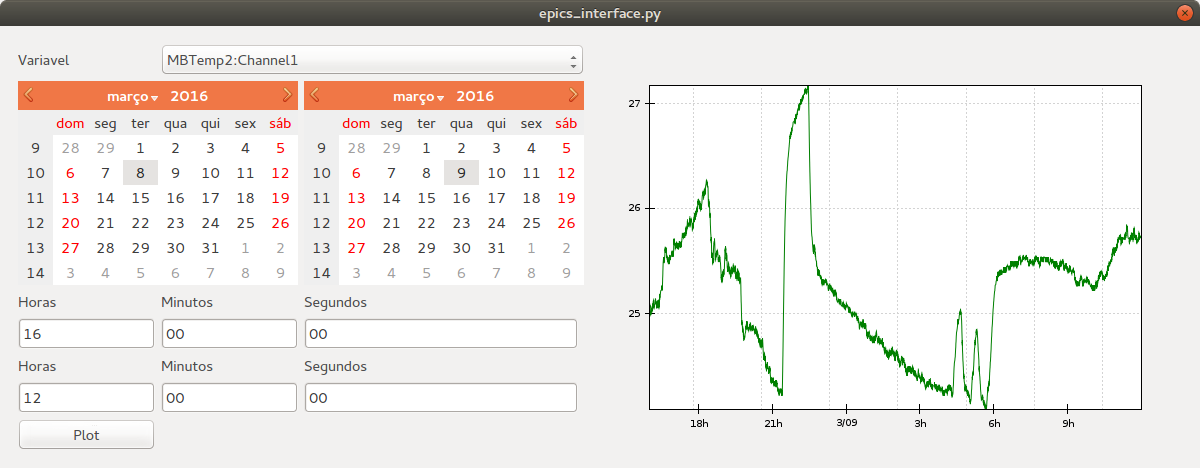
\includegraphics[scale=0.30]{image/screenshot-python}
    \caption {Interface \textit{Qt} implementada em \textit{python}.}
    \label{fig:interface} 
\end{figure} 